\subsection{Opdracht 02}
Geef het statement dat per land het maandgebruik over 12 maanden geeft met daarbij het percentage dat die maand uitmaakt van het totaal van die 12 maanden.
Hier zijn twee interpretaties mogelijk: per land de afgelopen 12 maanden in rijen, hier onder de uitdraai voor b.v. �Netherlands� uitgevoerd in april 2019.

\begin{lstlisting}
    Year	Month	ItemsPerMonth	PercentageOfTotal
    2018	4	    60		        4.44%
    2018	5	    60		        4.44%
    2018	6	    60		        4.44%
    2018	7	    56		        4.14%
    2018	8	    132		        9.76%
    2018	9	    155		        11.46%
    2018	10	    141		        10.43%
    2018	11	    138		        10.21%
    2018	12	    148		        10.95%
    2019	1	    137		        10.13%
    2019	2	    117		        8.65%
    2019	3	    148		        10.95%
\end{lstlisting}

\subsubsection{Versie 01}
De intentie was om een zo flexibel mogelijk query te schrijven. Zodat deze query ook makkelijk in gebruik
zou zijn wanneer de waardes van Country, Month of Year aangepast zou worden. Door gebruik te maken van de
Year en Month datetime functie, kunnen we alles purchases eruit filteren die we nodig hebben.
De basis data zetten we in een CTE, waar we daarna gebruik van maken om te groeperen en de percentages uit te rekenen.


\lstinputlisting[language=SQL]{sql/nick/opdracht-01-02a.sql}
\begin{figure}[H]
    \centering
    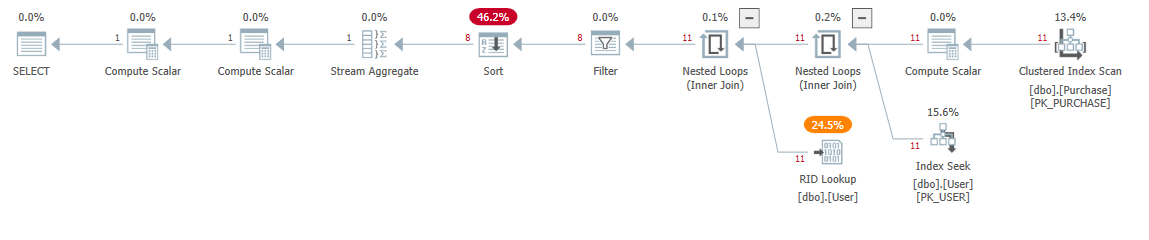
\includegraphics[width=1\textwidth]{image/nick/opdracht-02a.PNG}
    \caption{Queryplan Opdracht 02 Versie 01}
\end{figure}

\subsubsection{Versie 02}
    Bij de uitwerking van deze versie was het de intentie om resultaten van aankopen door verschillende gebruikers
    op te halen binnen een specifiek land en binnen een gestelde periode, zonder gebruik te maken van een CTE. Het jaar en de maand
    worden middels de YEAR en MONTH functies uit de gegevens ontrokken.

\lstinputlisting[language=SQL]{sql/marc/opdracht-01-02a.sql}
\begin{figure}[H]
    \centering
    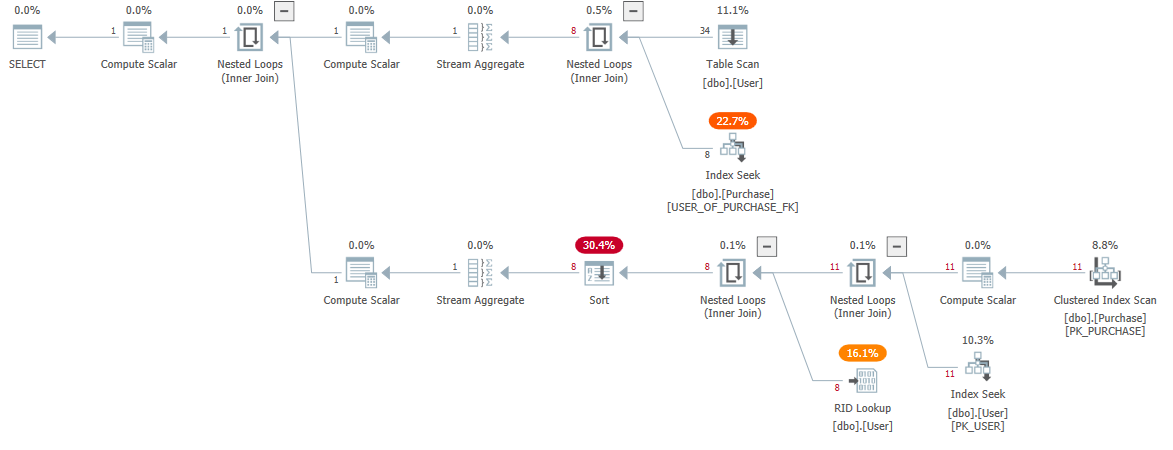
\includegraphics[width=1\textwidth]{image/marc/opdracht-02a.PNG}
    \caption{Queryplan Opdracht 02 Versie 02}
\end{figure}

\subsubsection{Versie 03}
TODO: Joey
\lstinputlisting[language=SQL]{sql/joey/opdracht-01-02a.sql}
\begin{figure}[H]
    \centering
    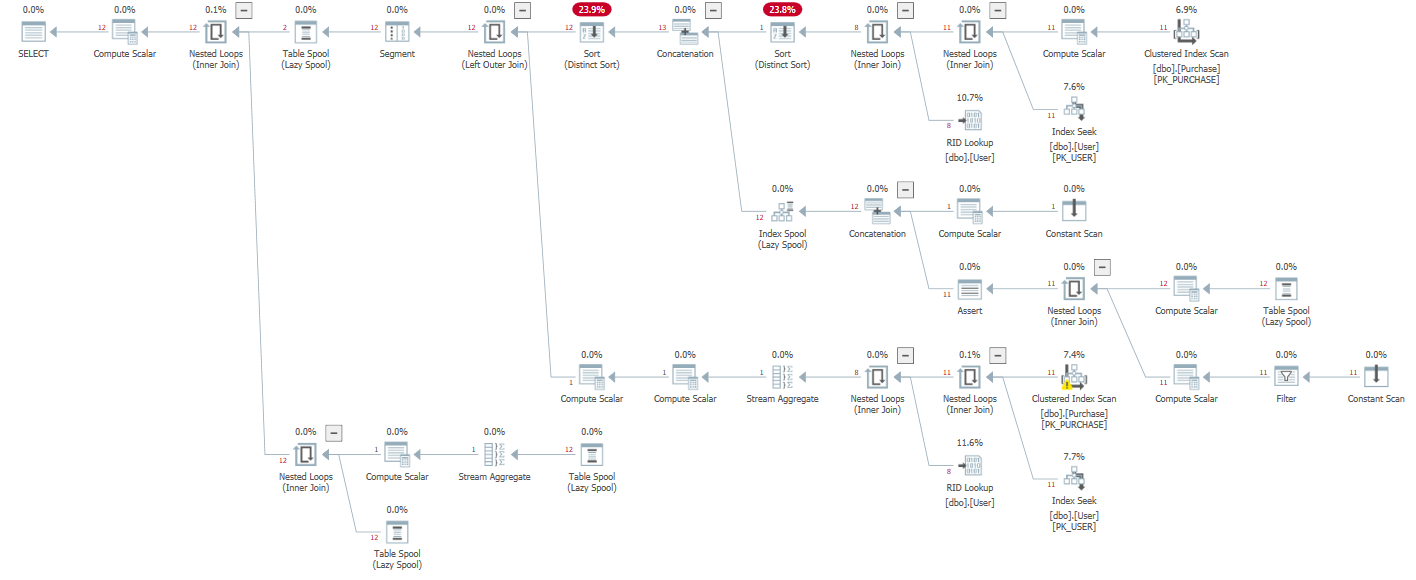
\includegraphics[width=1\textwidth]{image/joey/opdracht-02a.PNG}
    \caption{Queryplan Opdracht 02 Versie 03}
\end{figure}

\subsubsection{Conclusie}
Uit bovenstaande queryplannen is gebleken dat versie 01 en versie 02 qua 'cost relative to batch', gelijkwaardig presteren.
Wanneer deze gezamelijk in één batch worden uitgevoerd, tezamen met versie 03, nemen deze twee queries beiden 25% van de gehele
duur in beslag. Versie 03 neemt ruim 49\% van de gehele duur in beslag. De 'RID Lookup' van versie 01 presteert iets minder
snel aangezien deze voor alle records in de tabel User, de gegevens uit de kolommen van de tabel ophaalt. In versie 02 wordt
er in een eerder stadium al een onderscheid gemaakt. Hierdoor is de lijst met records waarvoor een 'RID Lookup' wordt gedaan bij
bij versie 02, in eerste instantie reeds verkleind tot de daadwerkelijke resulset waar we iets mee willen gaan doen. Kortom, doordat in
versie 02 niet alle gegevens van een User worden opgehaald, zal in de toekomst, zeker bij een groter aantal records in de tabel User,
versie 02 beter presteren dan versie 01.\\
\\
Het valt op dat versie 01 voorafgaand aan de 'Sort', een 'Filter' uitvoert. Dit komt voort uit het hierboven beschreven verschil.
Op dit moment wordt er bij versie 01 namelijk  pas onderscheid gemaakt tussen de records uit de tabel User. Voor alle records wordt
bepaald wat het land van de User is.\\
\\
Kijkende naar de opbouw van versie 01 en versie 02 kan worden gesteld dat versie 01 net wat prettiger leest dan versie 02.
Dit komt in dit geval voort uit het gebruik van de CTE waarbij een resultset wordt opgeleverd. Gezien de omvang van de query is dit
verschil echter beperkt en zijn beide queries eenvoudig te begrijpen. Het gebruikt van de CTE zorgt echter wel voor een minimale hoeveelheid
extra compile-time, namelijk ongeveer 10ms.\\
\\
De uiteindelijke conclusie luidt dat de verschillen tussen versie 01 en versie 02 op dit moment klein zijn, echter zal van bovenstaande
uitwerkingen versie 02 op termijn beter presteren. Beide queries zijn klein en de minimale winst die versie 02 op de compile-time heeft ten
opzichte van versie 01 is minimaal.\\
\\
\begin{tabular}{ || l | l | l | l | l | l | l | l | l | l | l | l | 1 | 1 | l | 1 | 1 || }
    \hline
    \textbf{Statement} & \textbf{Est Cost \%} & \textbf{Compile Time} & \textbf{Duration} &
    \textbf{CPU} & \textbf{Est CPU Cost \%} &
    \textbf{Est IO Cost \%} \\
    \hline
    \hline
    Versie01  & 25,4\%  & 26  & 1  & 1  & 27,2\% & 25,2\% \\
    \hline
    Versie02  & 25,4\%  & 16  & 1  & 1  & 27,2\% & 25,2\%  \\
    \hline
    Versie03  & 49,2\%  & 19  & 75  & 6  & 45,2\% & 49,5\%  \\
    \hline
\end{tabular}
\newline
\newline
\begin{tabular}{ || l | l | l | l | l | l | l | l | l | l | l | l | 1 | 1 | l | 1 | 1 || }
    \hline
    \textbf{Statement} &  \textbf{Est Rows} & \textbf{Actual Rows} & \textbf{RID Lookups} &
    \textbf{Parallel} & \textbf{Sort} &
    \textbf{Table Scan} & \textbf{Hash Match} \\
    \hline
    \hline
    Versie01  & 2  & 1  & 1  & 0  & 1  & 0  & 0 \\
    \hline
    Versie02  & 2  & 1  & 1  & 0  & 1  & 0  & 0 \\
    \hline
    Versie03  & 3  & 12  & 2  & 0  & 2  & 0  & 0 \\
    \hline
\end{tabular}